% Copyright (c) 2014,2016 Casper Ti. Vect
 
\chapter{相关理论与技术}
	
		⽐特币(Bitcoin,BTC)是⼀个点对点式的电⼦现⾦系统,集成了非对称式密钥密码学(Asymmetric Key Cryptography)\supercite{AsymmetricKeyCryptography}、签章密码学(Signature Cryptography)\supercite{Apublickeycryptosystemandasignatureschemebasedondiscretelogarithms}、零知识证明密码学(Zero Knowledge Proof Cryptography)\supercite{Zero-KnowledgeProofsofIdentity}、哈希函数密码学(Hash Function Cryptography)、共识算法(Consensus Algorithm)\supercite{Anonymousbyzantineconsensusfrommoderately-hardpuzzles:Amodelforbitcoin}诸多技术建构而成一个分布式、不需要仰赖中心化机构加以维护的交易帐本,表\ref{IntroductiontoBitcoin}是比特币系统的相关参数简介。在接下来的章节中将逐一进行详尽的说明每个技术在各个环节中所扮演的角色。

		\begin{table}[!htbp]
		\centering
		\caption{比特币系统的相关参数简介}
		\label{IntroductiontoBitcoin}
		\begin{tabular}{|l|l|}
		\hline
		第一个区块生成时间 & 2009年1月3日 \\ \hline
		比特币预计总产量 & 21,000,000 BTC \\ \hline
		比特币目前总产量 & 16,921,800 BTC \\ \hline
		最新区块高度 & 513743 块 \\ \hline
		比特币总市值 & 5兆 人民币 \\ \hline
		比特币全节点的数量 & 10552 个 \\ \hline
		单日比特币交易金额 & 124,017.02430718 BTC \\ \hline
		单日交易笔数 & 196,606 笔 \\ \hline
		比特币区块链大小 & 188.89 GB \\ \hline
		平均区块大小 & 0.75 MB \\ \hline
		平均生成单一区块所需时间 & 9.67 分钟 \\ \hline
		单日产出比特币数量 & 1,775 BTC \\ \hline
		挖矿难易度参数 & 3,290,605,988,755 \\ \hline
		全网挖矿算力 & 23,555,075.18 THash/s \\ \hline
		\end{tabular}
		\end{table}
		
		去中⼼化的加密货币系统给社会和传统中⼼化的⾦融体系以及政府带来了重⼤的冲击,Satoshi Nakamoto建构了一个不需要经过中央银行发行货币的货币系统,在比特币的货币发行上全靠区块链既定的算法。除了货币发行,也将交易记录的帐本以明文的方式存储在去中心化的区块链中,以比特币为例,现今完整的比特币区块链帐本已经高达180 GB,这样保存完整交易数据的计算机称之为全节点,在比特币去中心化的网络中,如图\ref{bitcoinfullnode}所示,截至2018年1月25比特币网络中全节点数量为10552个\supercite{bitcoinfullnode},全节点的数量决定了比特币帐本的可靠度,越多的全节点数量越能巩固⽐特币网络中过去的交易数据,使其难以被窜改。

		\begin{figure}
			\centering
			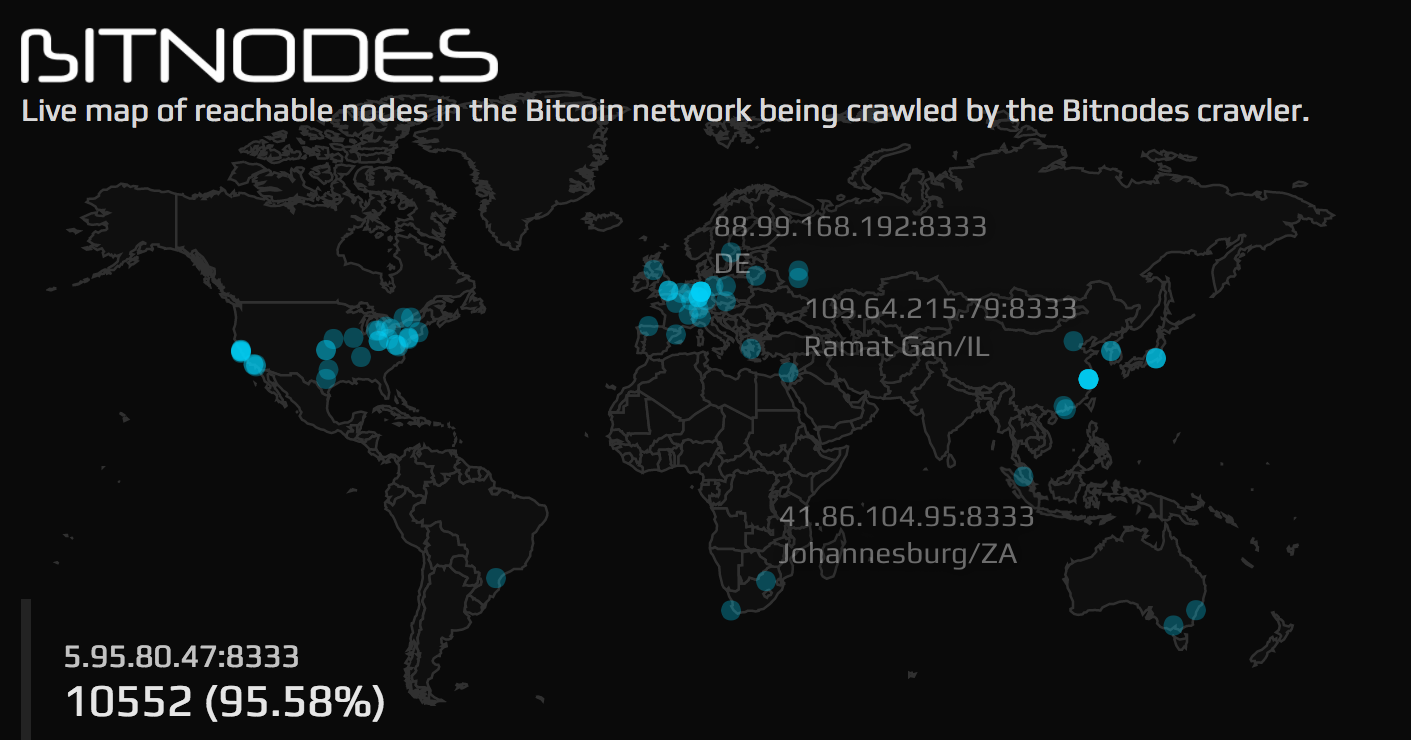
\includegraphics[width = .9\textwidth]{bitcoinfullnode.png}
			\caption{截至2018年2月17日止,⽐特币全节点分布图\supercite{bitcoinfullnode}}\label{bitcoinfullnode}
		\end{figure}


		\section{比特币地址}
		⽐特币地址为⽐特币的载体,深⼊了解⽐特币的地址⽣成相关算法、⽐特币地址⽣成过程、多重签章,可以近⼀步应⽤在比特币的交易监督系统。
		
		在点对点的现金系统中,首先必须先生成一个地址,在比特币的协议中有着既定的程序程序生成地址。运用到的技术包括乱数产生器(Random number generator)、非对称式加密算法Secp256k1\supercite{johnson2001elliptic}、哈希算法SHA-256\supercite{DBLP:conf/fse/KhovratovichRS12}以及Base58 编码\supercite{Base58}。接下来将详述每一个函数的运作过程以及意义,最后说明比特币交易地址生成的每一个步骤。
			
				\subsubsection{(一)乱数产生器(Random number generator)}
				乱数在密码学中是个相当重要的一环,在比特币系统中更是重要,毕竟生成的乱数会变成比特币的私钥,私钥是加密货币中是签署资产转移的唯一方式,在比特币地址中的乱数产生器会产出一个256 bits长度的乱数成为私钥,256 bits的长度可以表现的组态空间为$2^{256}$,换算成十进位表示为$1.1579209x10^{77}$,要在这组态空间中,以乱数产生同样的一把私钥是一件困难的事,但也有国际的实验室\supercite{TheLargeBitcoinCollider}团队正在努力的穷举比特币$2^{256}$的组态空间,如图\ref{LBC}所示,根据LBC公布的数据显示,目前已经完成了$2.330109x10^{16}$个地址探索。虽然$10^{16}$的级别与$10^{77}$的级别相距甚远,但LBC已探索的组态空间中击中了15个比特币地址,该团队也成功将这15 个地址下的1.180899个比特币转走。

				\begin{figure}[!htbp]
					\centering
					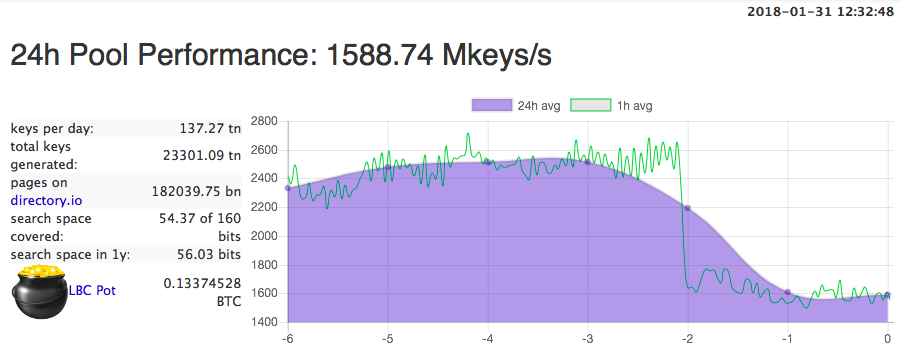
\includegraphics[width = .9\textwidth]{LBC.png}
					\caption{LBC穷举比特币私钥算力状态图\supercite{TheLargeBitcoinCollider}}\label{LBC}
				\end{figure}

				如何建构一个乱数,在过往的乱数产生器往往会加入时间作为参数,但对于一个攻击者而言,只需要去猜测在这段时间内目标者所有生成的可能性有极高的机率可猜出乱数。而乱数在密码学中常会是一把私钥的生成,在HTTPS 协议中,服务器端与客⼾端建⽴⼀个加密连接的过程中,也需要⼀个乱数去建⽴⾼安全性的加密信道-传输层安全性协定Transport Layer Security,TLS)\supercite{dierks2008transport},在SSH协议\supercite{ThesecureshellSSHprotocolarchitecture}中也采用了乱数。
		
				于2013 年8 ⽉⽐特币开发者Mike Hearn 于论文"All private keys generated on Android phones/tablets are weak and some signatures have been observed to have colliding R values"\supercite{SomeSecureRandomThoughts}中提及在过去的历史事件中,发现Android手持移动装置版以及平板版的乱数产生器中存在着不随机,在不同的手持移动装置中有机会生成同样的私钥。Bitcoin.org也发布了警告\supercite{AndroidSecurityVulnerability}简要说明该乱数不随机事件的原因,以及表明受到该事件影响的⽐特币钱包客⼾端包含有Bitcoin Wallet、BitcoinSpinner、Mycelium Bitcoin Wallet、blockchain.info。这样的错误源于Android本身支持的乱数产生器并不随机,随后Android解释了乱数的问题并加以修正。在这Android手持移动装置乱数不够乱的事件中,有自愿者自发性地公布自己的损失状态,总金额为55.82152538个比特币\supercite{Badsignaturesleading},但因为比特币属于被动的性质,无人主动回报即不会加入统计中,所以总损失估计会超过55.82152538个比特币。

				\subsubsection{(二)非对称式加密算法 Secp256k1}
				在密码学中有分对称式加密与非对称式加密,对称式加密又分为信息流加密与信息块加密,信息流加密著名的是由美国密码学家Ron Rivest教授发表,包括RC2(1987年)\supercite{OnthedesignandsecurityofRC2}、RC4(1987年)\supercite{Rc4}、RC5(1994年)\supercite{TheRC5encryptionalgorithm}、RC6(1998年)\supercite{TheRC6blockcipher.v1.1August201998};信息块加密著名的有数据加密标准(Data Encryption Standard,DES,1975年)\supercite{Dataencryptionstandard}、三重数据加密算法(Triple Data Encryption Algorithm,Triple DES,1998年)\supercite{TrippleDataEncryptionAlgorithmModesofOperation}、高级加密标准(Advanced Encryption Standard,AES,1998年)\supercite{ThedesignofRijndael:AES-theadvancedencryptionstandard};非对称式加密最广为人知的有RSA(Rivest–Shamir–Adleman,1977年)\supercite{Cryptographiccommunicationssystemandmethod}、椭圆曲线密码学(Elliptic curve cryptography,ECC,1985年)\supercite{Ellipticcurvecryptosystems}。
				非对称式加密与对称式加密最大的不同,在于对称式加密在加密解密的过程中只需要一把钥匙,而非对称式加密会生成两把钥匙,分别为私钥与公钥,在算法的设计上一开始会以乱数产生一把私钥,再经由非对称式加密算法推导出公钥,推导出的公钥在非对称式密码学中并无直接的方法可以反推至私钥,如此一来确立私钥的安全性。非对称式密码的使用场景有两种,第一种是希望收到加密信息的用户Alice,Alice会生成私钥存储在自己本地端的电脑中,并将推导出的公钥公布在网络上,这时希望联系Alice的用户Bob在网络上取得公钥后,Bob会以Alice的公钥进行加密,之后将密文寄送给Alice,在传递信息的过程中,即使网络存在着监听,也无法将信息顺利解密,唯有Alice收到信息后使用Alice原本产生该公钥的私钥,才可以解出明文。第二种则应用在比特币的交易之数字签名以及验证比特币交易,比特币地址的创建过程中会透过secp256k1生成私钥公钥对,在创建比特币交易的过程中,使用该地址的私钥对该地址未花费的输出(Unspent Transaction Output,UTXO)\supercite{bitcoinpaper}进行数字签名,完成数字签名后会与公钥以及交易信息一起广播到比特币网络的交易缓存池当中,比特币交易缓存池存在于所有比特币全节点当中,主要存储所有未被收录到比特币区块链内的所有交易,也就是零确认交易,等待矿工将该笔交易收入至比特币区块链当中。
				比特币采用的secp256k1是属于椭圆曲线密码学中的一个版本,不同的椭圆曲线版本的差异在于不同的初始参数,包括椭圆曲线方程$y^2=x^3+ax+b$、$p$=FFFFFFFFFFFFFFFFFFFFFFFFFFFFFFFFFFFFFFFFFFFFFFFFFFFFFFFEFFFFFC2F为巨大的素数、$G$点被称为⽣成点的常数点亦称为基点。至于为什么选择ECC而非RSA的主要原因,其一在于ECC在生成密钥对所需的时间更加快速,根据表\ref{ECCtime}显示,Nicholas Jansma于2004年针对ECC与RSA的密钥对生成时间与数字签名所需时间的论文\supercite{Performancecomparisonofellipticcurveandrsadigitalsignatures}显示,当ECC产生571 bits的密钥长度,要达到相同安全等级的情形下,RSA则需要⽣成15360 bits,这也让两种非对称式的加密方式之间,⽣成的时间产生了⾼达471 倍之差距。

				\begin{table}[!htbp]
				\centering
				\caption{ECC与RSA相同安全等级的密钥对生成时间比较表\supercite{Performancecomparisonofellipticcurveandrsadigitalsignatures}}
				\label{ECCtime}
				\begin{tabular}{|c|c|c|c|}
				\hline
				\multicolumn{2}{|c|}{密钥长度(bits)} & \multicolumn{2}{c|}{时间 (秒)} \\ \hline
				ECC & RSA & ECC & RSA \\ \hline
				163 & 1024 & 0.08 & 0.16 \\ \hline
				33 & 2240 & 0.18 & 7.47 \\ \hline
				283 & 3072 & 0.27 & 9.8 \\ \hline
				409 & 7680 & 0.64 & 133.9 \\ \hline
				571 & 15360 & 1.44 & 679.06 \\ \hline
				\end{tabular}
				\end{table}	

				除了在密钥对生成时间ECC有着比RSA更高效的算法外,在安全性上ECC可以更短的密钥长度达到与RSA相同的安全强度,Léo Ducas针对ECCRSA、BLISS(Bimodal Lattice Signature Scheme)\supercite{LatticesignaturesandbimodalGaussians}做出了深度的安全性探讨,表\ref{LatticesignaturesandbimodalGaussians}同样达到80 bits的安全性级数,RSA 1024需要1024 bits,ECDSA 160\supercite{DeploymentsofEllipticCurveCryptography}仅需要160 bits,该篇论文除了探讨RSA与ECDSA(Elliptic Curve Digital Signature Algorithm)之外,更大的部分在阐述量子计算机对于既有的传统密码带来的抨击,有机会快速穷举$2^{256}$的比特币私钥,在未来量子计算机的蓬勃发展拥有2000 qbits运算能力,量子计算机可以快速穷举破解所有的比特币私钥。因此发展针对量子计算机设计的数字签名算法成为密码学上崭新的议题,而BLISS则为针对量子计算机所设计的抗量子计算的签章算法。

				\begin{table}[!htbp]
				\centering
				\caption{算法BLISS、RSA、ECDSA安全级数比较图表\supercite{LatticesignaturesandbimodalGaussians}}
				\label{LatticesignaturesandbimodalGaussians}
				\resizebox{\textwidth}{!}{%
				\begin{tabular}{|c|c|c|c|c|c|c|c|c|}
				\hline
				算法 & 安全性 & \begin{tabular}[c]{@{}c@{}}签名\\ 大小\end{tabular} & \begin{tabular}[c]{@{}c@{}}私钥\\ 大小\end{tabular} & \begin{tabular}[c]{@{}c@{}}公钥\\ 大小\end{tabular} & \begin{tabular}[c]{@{}c@{}}签名\\(微秒)\end{tabular} & 签名/秒 & \begin{tabular}[c]{@{}c@{}}验证\\(微秒)\end{tabular} & 验证/秒 \\ \hline
				BLISS-0 & $\leq$60 bits & 3.3 kb & 1.5 kb & 3.3 kb & 0.241 & 4k & 0.017 & 59k \\ \hline
				BLISS-I & 128 bits & 5.6 kb & 2 kb & 7 kb & 0.124 & 8k & 0.03 & 33k \\ \hline
				BLISS-II & 128 bits & 5 kb & 2 kb & 7 kb & 0.48 & 2k & 0.03 & 33k \\ \hline
				BLISS-III & 160 bits & 6 kb & 3 kb & 7 kb & 0.203 & 5k & 0.031 & 32k \\ \hline
				BLISS-IV & 192 bits & 6.5 kb & 3 kb & 7 kb & 0.375 & 2.5k & 0.032 & 31k \\ \hline
				RSA-1024 & 72-80 bits & 1 kb & 1 kb & 1 kb & 0.167 & 6k & 0.004 & 91k \\ \hline
				RSA-2048 & 103-112 bits & 2 kb & 2 kb & 2 kb & 1.18 & 0.8k & 0.038 & 27k \\ \hline
				RSA-4096 & $>$128 bits & 4 kb & 4 kb & 4 kb & 8.66 & 0.1k & 0.138 & 7.5k \\ \hline
				ECDSA-160 & 80 bits & 0.32 kb & 0.16 kb & 0.16 kb & 0.058 & 17k & 0.205 & 5k \\ \hline
				ECDSA-256 & 128 bits & 0.5 kb & 0.25 kb & 0.25 kb & 0.106 & 9.5k & 0.384 & 2.5k \\ \hline
				ECDSA-384 & 192 bits & 0.75 kb & 0.37 kb & 0.37 kb & 0.195 & 5k & 0.853 & 1k \\ \hline
				\end{tabular}%
				}
				\end{table}

				\subsubsection{(三)哈希算法 SHA-256}
				SHA-256是SHA(Secure Hash Algorithm,FIPS 182-2)\supercite{DBLP:conf/fse/KhovratovichRS12}哈希算法的家族之一。SHA家族当中有着四大分支,分别为SHA-0、SHA-1、SHA-2和SHA-3。各种哈希算法的差异在于运算初始变量、算法所采用的运算子、接受的信息长度以及循环数的不同,如表\ref{hashtable}所示。上述的参数差异皆由联邦信息处理标准(Federal Information Processing Standards,FIPS)中定义。表\ref{hashtable}中MD5不为SHA家族成员之一,但MD5为最早被广泛使用的哈希算法,因此此表将其作为借鉴的标准。SHA-0为SHA家族中被最早提出的架构,输出的长度为160 bits,而SHA-1提出后并无太大的变动。
				哈希算法的主要功能在于将信息或是文件建⽴专属的对应指纹,也就是哈希值,依照不同的算法设计,该指纹的输出⾧度也略有不同,表\ref{hashtable}显示了MD5与SHA 家族的输出哈希值⾧度,而长度也意味着该指纹的组态空间所映射的大小。倘若有着不同的输入,但映射到了相同的指纹,则将此现象称之为碰撞。通常在信息安全领域中,只要发现该哈希算法存在着碰撞,就会被弃用。有些专家甚⾄会提早数年建议用户尽早更换该哈希算法,并更换上新制定的哈希算法做应⽤。哈希算法的功能包括借由生成哈希值进行文件校验、工作量证明算法设计以及区块链中的哈希指针\supercite{Double-spendAttackModelswithTimeAdvantangeforBitcoin}。

				\begin{table}[!htbp]
					\centering
					\caption{MD5、SHA-0、SHA-1、SHA-2和SHA-3比较表}
					\label{hashtable}
					\begin{tabular}{|c|c|c|c|c|c|c|}
					\hline
					算法 & 分支 & \begin{tabular}[c]{@{}c@{}}输出\\ 哈希值\\ 长度\\ (bits)\end{tabular} & \begin{tabular}[c]{@{}c@{}}最大输入\\ 信息长度\\ (bits)\end{tabular} & \begin{tabular}[c]{@{}c@{}}循环\\ (次数)\end{tabular} & 使用到的运算子 & \begin{tabular}[c]{@{}c@{}}碰撞\\ 攻击\\ (bits)\end{tabular} \\ \hline
					\begin{tabular}[c]{@{}c@{}}MD5\\ 参考\end{tabular} & - & 128 & $\infty$ & 64 & \multirow{3}{*}{\begin{tabular}[c]{@{}c@{}}And, Xor, Rot, Or, \\ Add (mod $2^{32}$)\end{tabular}} & \begin{tabular}[c]{@{}c@{}}$<64$ \\ 已碰撞\end{tabular} \\ \cline{1-5} \cline{7-7} 
					SHA-0 & - & \multirow{2}{*}{160} & \multirow{2}{*}{$2^{64}-1$} & \multirow{2}{*}{80} &  & \begin{tabular}[c]{@{}c@{}}$<80$ \\ 已碰撞\end{tabular} \\ \cline{1-2} \cline{7-7} 
					SHA-1 & - &  &  &  &  & \begin{tabular}[c]{@{}c@{}}$<80$ \\ 已碰撞\end{tabular} \\ \hline
					\multirow{4}{*}{SHA-2} & SHA-224 & 224 & \multirow{2}{*}{$2^{64}-1$} & \multirow{2}{*}{64} & \multirow{2}{*}{\begin{tabular}[c]{@{}c@{}}And, Xor, Rot, Or, Shr, \\ Add (mod $2^{32}$)\end{tabular}} & 112 \\ \cline{2-3} \cline{7-7} 
					 & SHA-256 & 256 &  &  &  & 128 \\ \cline{2-7} 
					 & SHA-384 & 384 & \multirow{2}{*}{$2^{128}-1$} & \multirow{2}{*}{80} & \multirow{2}{*}{\begin{tabular}[c]{@{}c@{}}And, Xor, Rot, Or, Shr, \\ Add (mod $2^{64}$)\end{tabular}} & 192 \\ \cline{2-3} \cline{7-7} 
					 & SHA-512 & 512 &  &  &  & 256 \\ \hline
					\multirow{4}{*}{SHA-3} & SHA3-224 & 224 & \multirow{4}{*}{$\infty$} & \multirow{4}{*}{24} & \multirow{4}{*}{And, Xor, Rot, Not} & 112 \\ \cline{2-3} \cline{7-7} 
					 & SHA3-256 & 256 &  &  &  & 128 \\ \cline{2-3} \cline{7-7} 
					 & SHA3-384 & 384 &  &  &  & 192 \\ \cline{2-3} \cline{7-7} 
					 & SHA3-512 & 512 &  &  &  & 256 \\ \hline
					\end{tabular}
					\end{table}

				\begin{enumerate}
				\item 生成哈希值进行文件校验:哈希值在过往的应用中,往往作为文件完整性的校验,软件供应方会在网站中提供各式不同算法的哈希值,让使⽤者在下载完软件之后输⼊使⽤者方以哈希算法所⽣成的哈希值进⾏⽐对。但倘若该哈希算法存在碰撞的发生,这会使得不同的文件存在着同样的哈希值。这也意味着软件供应方所提供的软件可能存在着掺入恶意代码后,还能生成同样的哈希指纹,失去了文件完整性的校验功能,这便成为信息安全中的重大漏洞,由表\ref{hashtable}可以看出软件提供方若使用MD5、SHA-0以及SHA-1会造成发生碰撞导致指纹失去校验意义成为安全漏洞,因此MD5、SHA-0以及SHA-1已被弃用。

				\item 工作量证明算法设计:起初工作量证明算法的概念为设计一个相当困难耗时的解,但验算的过程中却相当简单快速。如对一个大数做因式分解是一个相当困难的事,但要验算其结果仅需要将所有的解相乘确认是否为该大数即可证明。同样的理念在比特币系统中是以hash-puzzle的方式实现,hash-puzzle是利用哈希函数有着不可预期的特性,不可预期指的是假设输入连续性的数值$1$到$n$进入到哈希函数生成哈希值,而生成的哈希值无法观察出关联性,可说是完全不相关的数值,且无法预期下个输入的输出哈希值。
				比特币系统中的困难度变量,在hash-puzzle中定义了何谓真正的答案。在SHA-256当中输出的值为256 bits的哈希值,困难度变量则规定了在这256 bits当中,自最左边起必须为零的位数的门槛,而在困难度变量要求必须为零的位数变多,则意味着要在连续性的数值$1$到$n$的hash-puzzle中,符合门槛的解越少。在hash-puzzle中,求得一个符合困难度变量的哈希值是困难的,但要验算求得的解是否符合困难度的门槛相当快速,这符合起初工作量证明算法的概念。

				\begin{figure}[!htbp]
					\centering
					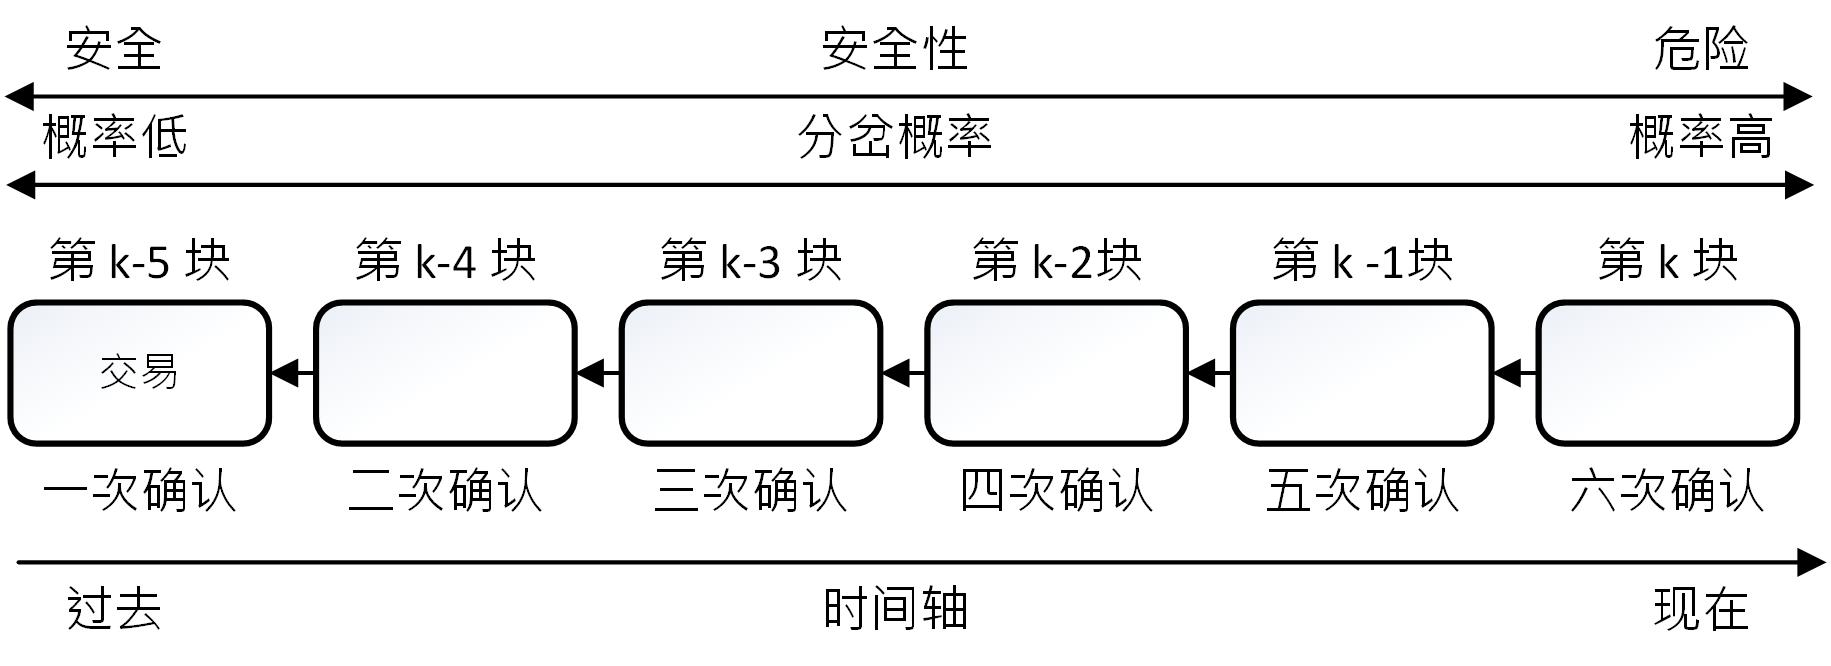
\includegraphics[width = 0.8\textwidth]{6confirm.jpg}
					\caption{区块叠加示意图}\label{6confirm}
				\end{figure}

				\item 区块链中的哈希指针:比特币区块链的区块头当中,当前区块存储着前区块头的双重哈希的哈希值。当前区块则会如数据结构链结串列一样,直到链结到第一个比特币区块的创世区块,区块链中的哈希指针将区块链结在一起,也就形成了比特币区块链的基础。在比特币挖矿的过程中,矿工参与着最新区块的hash-puzzle解题,寻找一个符合困难度变量的输入。但hash-puzzle 的工作证明当中解可能不只一个,但只要符合困难度变量的解都可以创建一个新的区块,届时就会在当前的区块上同时产生分岔,分岔的区块在比特币系统中皆为有效,但经过多个区块的叠加之后,便可以抉择出最长的链,该最长链则成为主链,而其他的分岔链,则成为孤儿块被丢弃,当中曾记载的交易信息变为无效,造成该分岔链的交易信息回溯。比特币区块链的分岔好发于最新的区块,如图\ref{6confirm}所示,而越旧的区块则越不易发生,所以在比特币交易中默认该笔交易要在六个区块确认后,该公司才会承认该笔交易有效。

				\end{enumerate}

				

					

	%			\subsubsection{RIPEMD-160}
				\subsubsection{(四)Base58 编码}

				表\ref{Base58}为Base58编码表,Base58编码的首次出现自Satoshi Nakamoto所提出的论文\supercite{bitcoinpaper}当中,Base58编码是源自于Base64编码表,如表\ref{Base64}中所示。Base64编码中包括大写英文26个字母、小写英文26个字母、阿拉伯数字以及字符"/"和"+"。在比特币地址生成过程中,Base58的功能是将比特币地址的公钥哈希值重新编码,比特币地址的公钥哈希值是二进制的数据型态,既使是将二进制码转换成十六进制码输出也是对人类辨识上有一定的不便性。倘若采用Base64对比特币公钥哈希值进行编码有效缩短二进制码的长度,但Base64的编码存在着不适于作为地址的特殊字符"+"和"-"。在Base58编码中移除了特殊字符"+"和"-"之外,也移除了⼈类较不易判读的相关字符,数字"0"与大写英文字母"O",因为该两字符在不同字体的体现相当相似,大写英文字母"I"以及小写英文字母"l",在人类判读上也有些为相似。因此于Base64移除上述6个字符后,便形成了Base58编码表。值得一提的是,Base58编码与Base64编码表中的字符排序有些许异动,Base58编码表将数字的部分移置到最前面,这也是比特币地址在以Base58编码后所呈现的第一个字符为"1"的主要原因。

					\begin{table}[!htbp]
					\centering
					\caption{Base58 编码表}
					\label{Base58}
					\begin{tabular}{|c|c|c|c|c|c|c|c|}
					\hline
					数值 & 字符 & 数值 & 字符 & 数值 & 字符 & 数值 & 字符 \\ \hline
					0 & 1 & 16 & H & 32 & Z & 48 & q \\ \hline
					1 & 2 & 17 & J & 33 & a & 49 & r \\ \hline
					2 & 3 & 18 & K & 34 & b & 50 & s \\ \hline
					3 & 4 & 19 & L & 35 & c & 51 & t \\ \hline
					4 & 5 & 20 & M & 36 & d & 52 & u \\ \hline
					5 & 6 & 21 & N & 37 & e & 53 & v \\ \hline
					6 & 7 & 22 & P & 38 & f & 54 & w \\ \hline
					7 & 8 & 23 & Q & 39 & g & 55 & x \\ \hline
					8 & 9 & 24 & R & 40 & h & 56 & y \\ \hline
					9 & A & 25 & S & 41 & i & 57 & z \\ \hline
					10 & B & 26 & T & 42 & j &  &  \\ \hline
					11 & C & 27 & U & 43 & k &  &  \\ \hline
					12 & D & 28 & V & 44 & m &  &  \\ \hline
					13 & E & 29 & W & 45 & n &  &  \\ \hline
					14 & F & 30 & X & 46 & o &  &  \\ \hline
					15 & G & 31 & Y & 47 & p &  &  \\ \hline
					\end{tabular}
					\end{table}

					\begin{table}[!htbp]
					\centering
					\caption{Base64 编码表}
					\label{Base64}
					\begin{tabular}{|c|c|c|c|c|c|c|c|}
					\hline
					数值 & 字符 & 数值 & 字符 & 数值 & 字符 & 数值 & 字符 \\ \hline
					0 & A & 16 & Q & 32 & g & 48 & w \\ \hline
					1 & B & 17 & R & 33 & h & 49 & x \\ \hline
					2 & C & 18 & S & 34 & i & 50 & y \\ \hline
					3 & D & 19 & T & 35 & j & 51 & z \\ \hline
					4 & E & 20 & U & 36 & k & 52 & 0 \\ \hline
					5 & F & 21 & V & 37 & l & 53 & 1 \\ \hline
					6 & G & 22 & W & 38 & m & 54 & 2 \\ \hline
					7 & H & 23 & X & 39 & n & 55 & 3 \\ \hline
					8 & I & 24 & Y & 40 & o & 56 & 4 \\ \hline
					9 & J & 25 & Z & 41 & p & 57 & 5 \\ \hline
					10 & K & 26 & a & 42 & q & 58 & 6 \\ \hline
					11 & L & 27 & b & 43 & r & 59 & 7 \\ \hline
					12 & M & 28 & c & 44 & s & 60 & 8 \\ \hline
					13 & N & 29 & d & 45 & t & 61 & 9 \\ \hline
					14 & O & 30 & e & 46 & u & 62 & + \\ \hline
					15 & P & 31 & f & 47 & v & 63 & / \\ \hline
					\end{tabular}
					\end{table}
	%
			于上述章节中已经详细说明⽐特币地址⽣成过程中使⽤到的所有相关算法技术,以及算法在现今的⽐特币系统中存在的问题。于本节中将阐述如何将比特币地址生成的相关算法实际带入比特币地址生成的过程中,地址的生成总共分为八个步骤,分别为生成私钥、生成公钥、生成公钥SHA-256 、生成公钥SHA-256 的RIPEMD-160 、取得版本号、生成校验码、版本号与公钥SHA-256的RIPEMD-160和校验码合并,最后一步则是将合并的结果以Base58编码创建出一个比特币地址。

			\begin{figure}[!htbp]
					\centering
					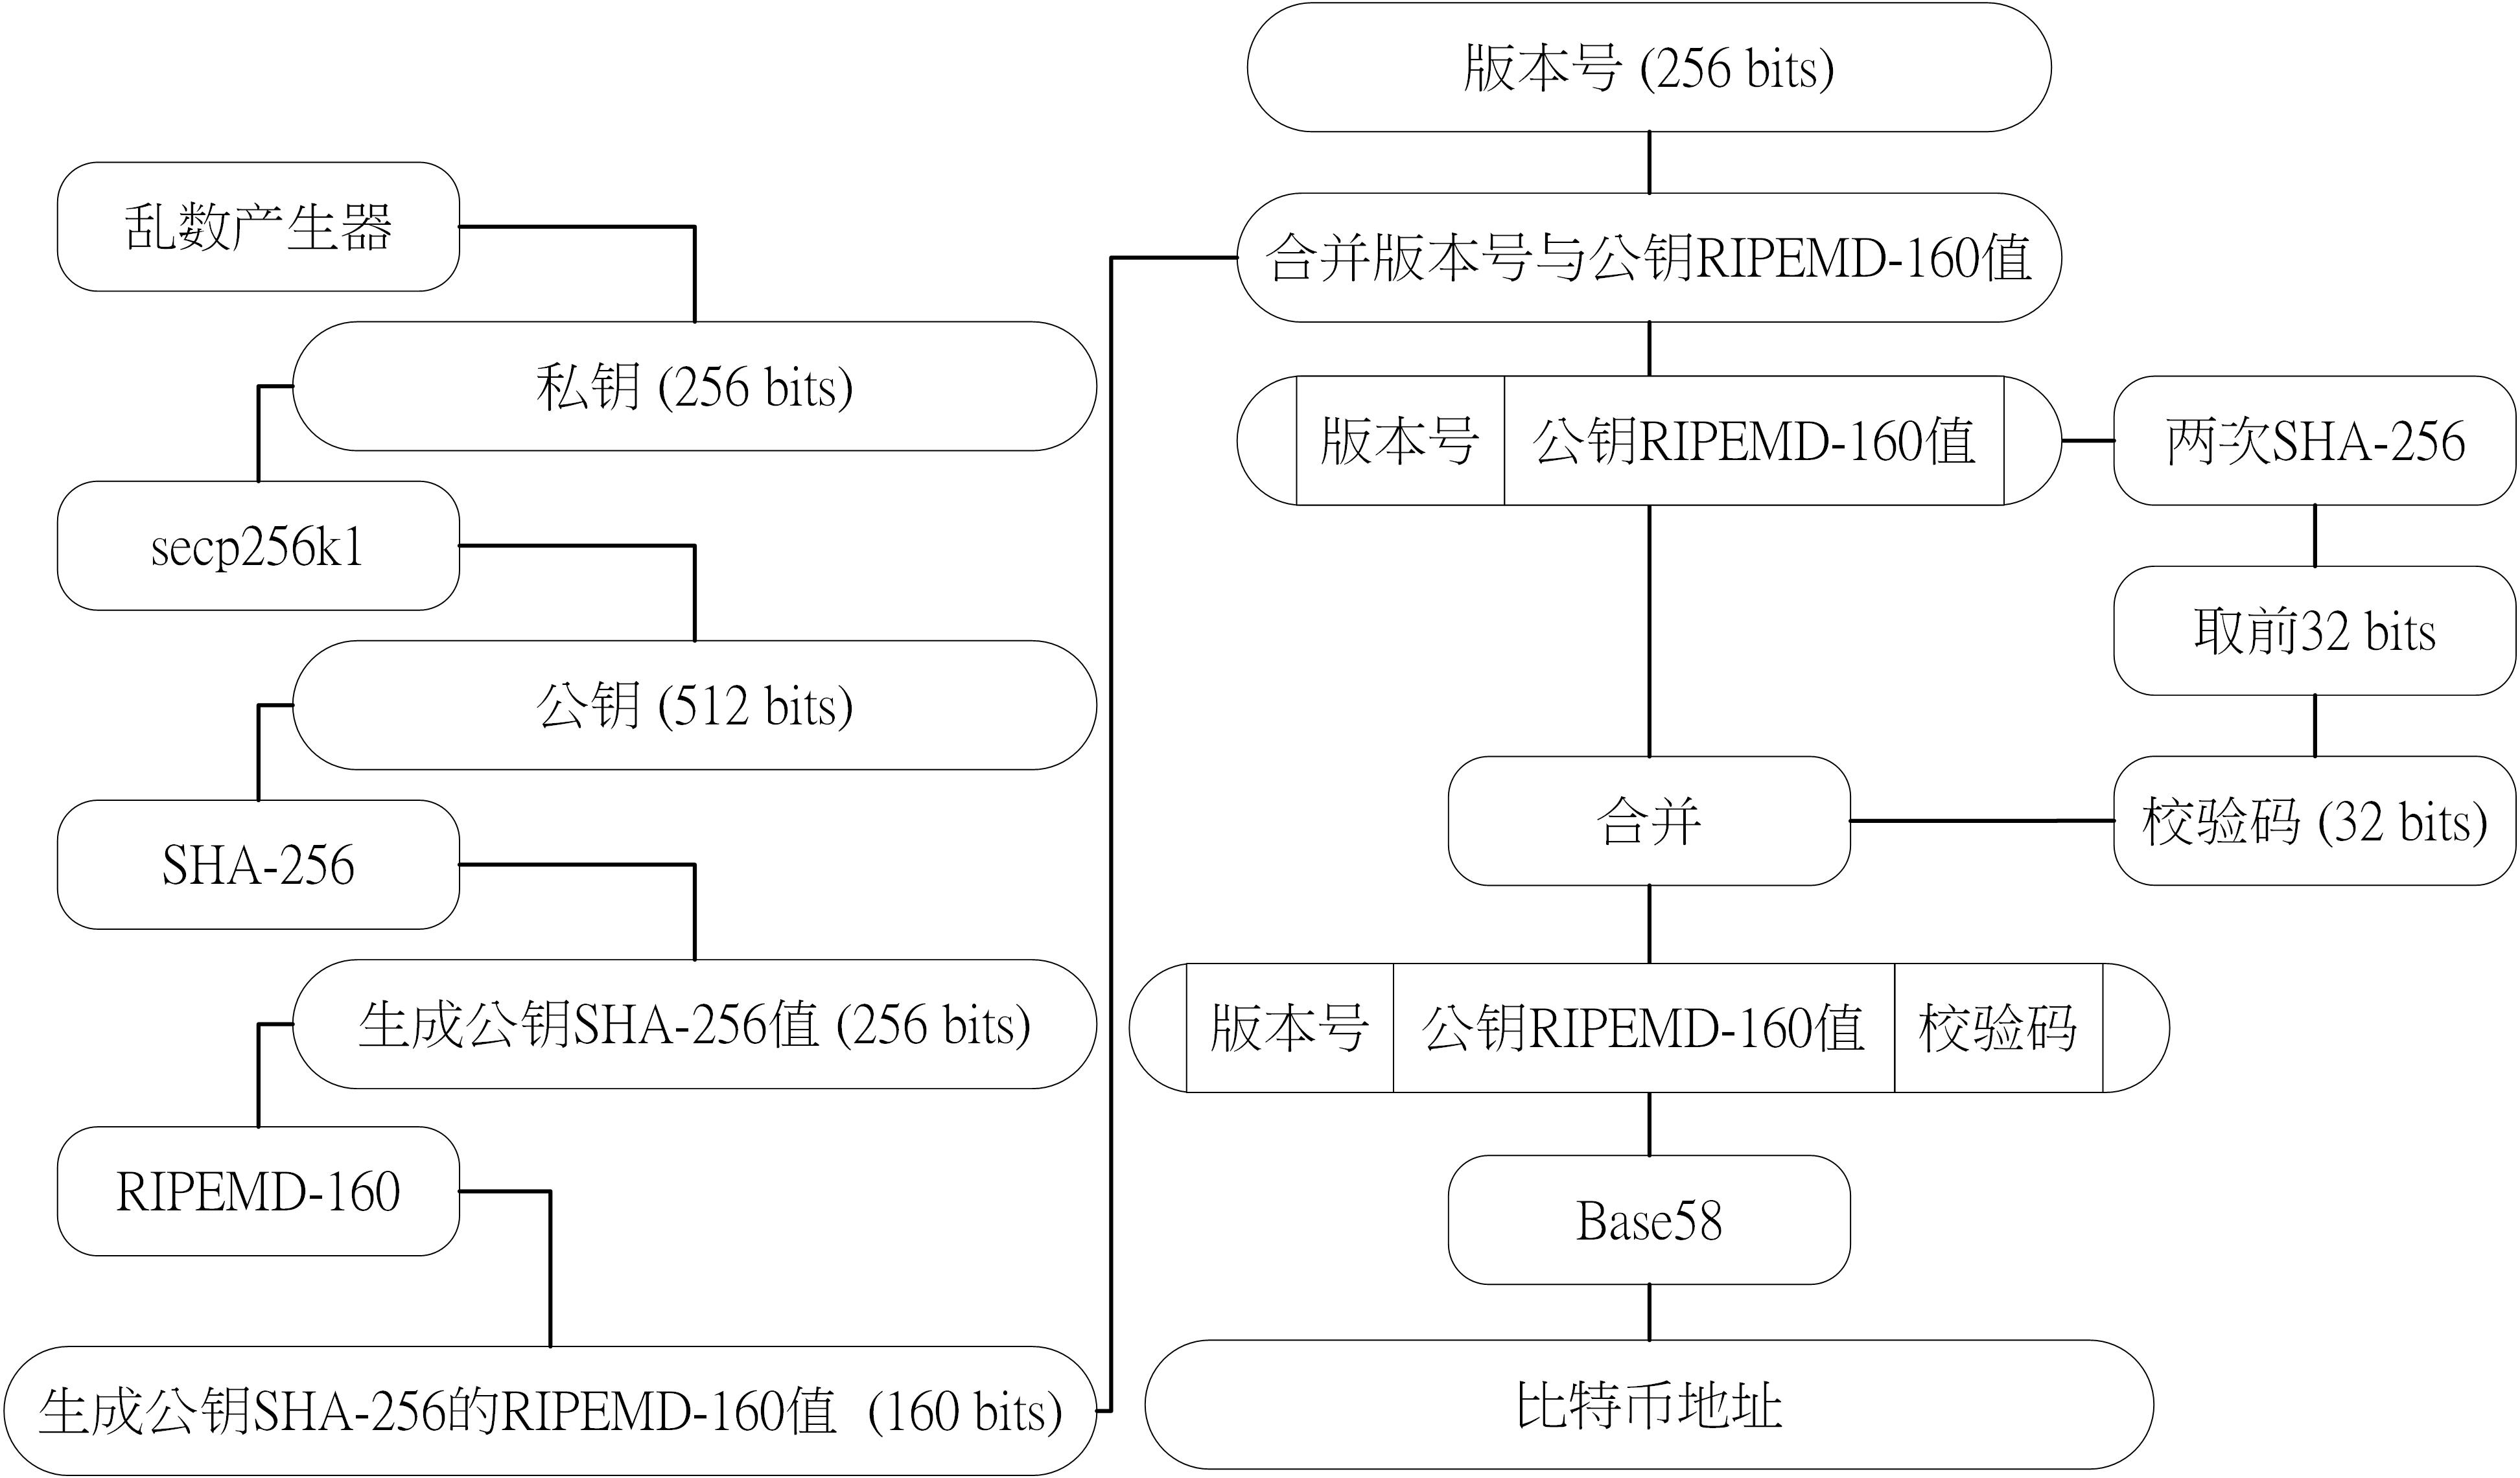
\includegraphics[width = .9\textwidth]{address.jpg}
					\caption{比特币地址生成流程图}\label{address}
			\end{figure}

			\begin{enumerate}
				\item 生成私钥:使用乱数产生器产生一个长度为256 bits的乱数,而此乱数即成为该比特币地址的私钥。在比特币的系统当中,私钥可以透过椭圆曲线签章算法secp256k1签署一笔交易,广播到⽐特币网络当中。由于私钥为该地址资金转移的关键,黑客攻击的对象皆会聚焦在比特币私钥,因此私钥的保存成为比特币系统中最为热门的课题之一。
				\item 生成公钥:在以乱数产生器生成私钥之后,接下来将运用到非对称式密码学中的私钥公钥转换算法,于比特币系统中采用的是secp256k1
				,secp256k1 是椭圆曲线密码学中的其中一个版本,不同的版本差异在于采用不同的变量。于比特币地址生成的过程中,secp256k1 负责将上述步骤所生成的私钥透过椭圆曲线算法计算出公钥,生成的公钥长度为512 bits,这比第一个步骤所生成的 256 bits 私钥多出⼀倍的⾧度。在比特币交易中,私钥可以签署一笔交易,在签署完之后便会将公钥、签名以及交易信息广播至比特币网络中,等待被收入到比特币区块链当中。此时该笔交易在⽐特币交易缓存池中等待secp256k1 算法对其公钥、签名以及交易信息进⾏验算,若计算出的值为真,则该笔交易被视为有效且继续待在交易缓存池中,等待被收⼊区块链内。
				\item 生成公钥SHA-256 :SHA-256 为SHA家族之一,也是哈希算法的一种,因此符合哈希算法的特征包括雪崩效应、不可预测、不可逆(单向性)以及校验文件是否完整的诸多特性。将前一个步骤所⽣成的⾧度为512 bits 的公钥作为SHA-256的输入,产出长度仅为公钥一半的公钥SHA-256哈希值。这个步骤将使即使知道公钥SHA-256的攻击者,更难以⽤穷举攻击推导出该地址的公钥。
				\item 生成公钥SHA-256 的RIPEMD-160 :RIPEMD-160 也是哈希算法的⼀种,和其他哈希算法的特征相符,与SHA-256 不同的部分在于RIPEMD-160 所⽣成的哈希值⾧度为160 bits。在前一步骤中进⾏SHA-256 计算的公钥已经有了第⼀层的保护,⽽在第四个步骤中,再次透过RIPEMD-160 取得哈希值。这将使得攻击者既使取得了⽐特币地址,也必须先针对RIPEMD-160 进⾏破译,再进⼀步对SHA-256 破译,才有机会取得该地址的公钥。因为这样的设计,让只收取却不花费的⽐特币地址,在⿊客攻击上造成相当⼤的难度。
				\item 取得版本号:在比特币系统初始的设计中,已经定义了些不同功能的比特币地址,这些特殊功能的比特币地址有着特殊的版本号,最为常见的为以"1"为头的比特币地址,该地址为比特币系统中最早被使用且最为普遍的地址版本,该种地址为一把私钥进行比特币地址推倒,所以仅需要一把钥匙就可以移动该地址下的比特币资产;第二种是以"3"为地址开头的比特币地址,该地址采用多重签章技术,该技术为后续经过多项BIP才完成落实于比特币系统。在第五个步骤中会加入版本号加以区分不同的地址。
				\item 生成校验码:校验码是⽐特币地址⽣成过程中重要的⼀环。校验码可降低⽐特币的⽀付过程中因⼿误而转⼊到不存在(不符合⽐特币地址⽣成规则)地址的可能性。在第六个步骤中对公钥SHA-256 的RIPEMD-160 再做两次SHA-256 ,取该哈希值前32 bits 的值作为校验码。
				\item 版本号与公钥SHA-256 的RIPEMD-160 和校验码合并:即将第五步骤产⽣的版本号、第四个步骤产⽣的公钥RIPEMD-160 及第六个步骤产⽣之校验码三者进行合并。
				\item 合并的结果以Base58 编码:Base58 修改⾃Base64 ,其与Base64 最⼤不同之处在于移除了"0"、"O"、"I"、"l"、"+"、"/"的字符,可以降低⼈⼯在判读地址的错误率。在这个步骤中使⽤Base58 将第七步骤合并的组合结果进⾏编码。
			\end{enumerate}

			 	比特币区块链技术,虽然已经利用工作量证明的方式解决了双重支付(Double-spending)问题\supercite{Informationpropagationinthebitcoinnetwork}\supercite{Double-spendingfastpaymentsinbitcoin},但工作量证明的算法所设置之题目困难度会直接影响到每一个比特币区块的产出时间,这个比特币区块的产出时间也考虑到比特币全节点于全世界各地的网络同步状况,倘若今天的区块生成时间过短会造成全世界的比特币节点之区块数据不一致,这样的数据不一致将导致比特币区块链出现分岔,再更严重一点甚至会造成比特币网络的瓦解。

			 	现今的⽐特币区块产出速度为⼗分钟⼀块,附上⾜够的⼿续费也须等待将近⼗分钟的交易时间,若是在⼿续费较低的情况下,该笔⽐特币交易甚⾄可能会在交易缓存池中滞留⼀周的时间才被矿工运算。即使在⼿续费⾜够的情况下,⼗分钟的确认时间会对实体商家的⼩额交易处理⾮常不友善,为了在既有的⽐特币区块链框架底下能够提升交易速度,因此产生了多重签章(Multi-Signature)技术。多重签章于在交易开始创建的同时管控双重⽀付交易的发⽣,采⽤了2-of-2 多重签章创建⼀个特殊的⽐特币地址,这个地址由两个代表⼈所持有,分别为使⽤者与Green Address\supercite{GreenAddress}机构节点,每笔交易的建⽴必须要双⽅同时签署才被允许广播⾄⽐特币网络中。若是遇到交易塞⾞,且节点缓存池空间不⾜的情况时,⽐特币节点会优先遗弃⼿续费最低的交易,视同该笔交易不曾存在过。若真的遇到交易被遗弃的情况,Green Address 机构节点也会在之后透过内部的数据库记录再次广播此笔交易,并确保此笔交易可以被收⼊⾄区块内。Green Address 机构节点因此成为了交易创建的把关者,过滤所有双重⽀付攻击的发⽣,也避免交易因为⽐特币网络塞⾞⽽被矿⼯遗弃的情形。在这样的机制下,只要是使⽤Green Address 钱包交易就可避免双重⽀付攻击的发⽣,对商家或是收款⼈⽽⾔,可以在即时交易中同时得到双重⽀付攻击的保护,也提高了交易在未进⼊区块链前的可确定性,达到即时交易的可能。

			 	\subsubsection{(一)Green Address钱包生成过程}
			 	此节将详细阐述Green Address钱包生成过程的重要步骤,如图\ref{gabuild}所示。
			 	\begin{figure}[!htbp]
					\centering
					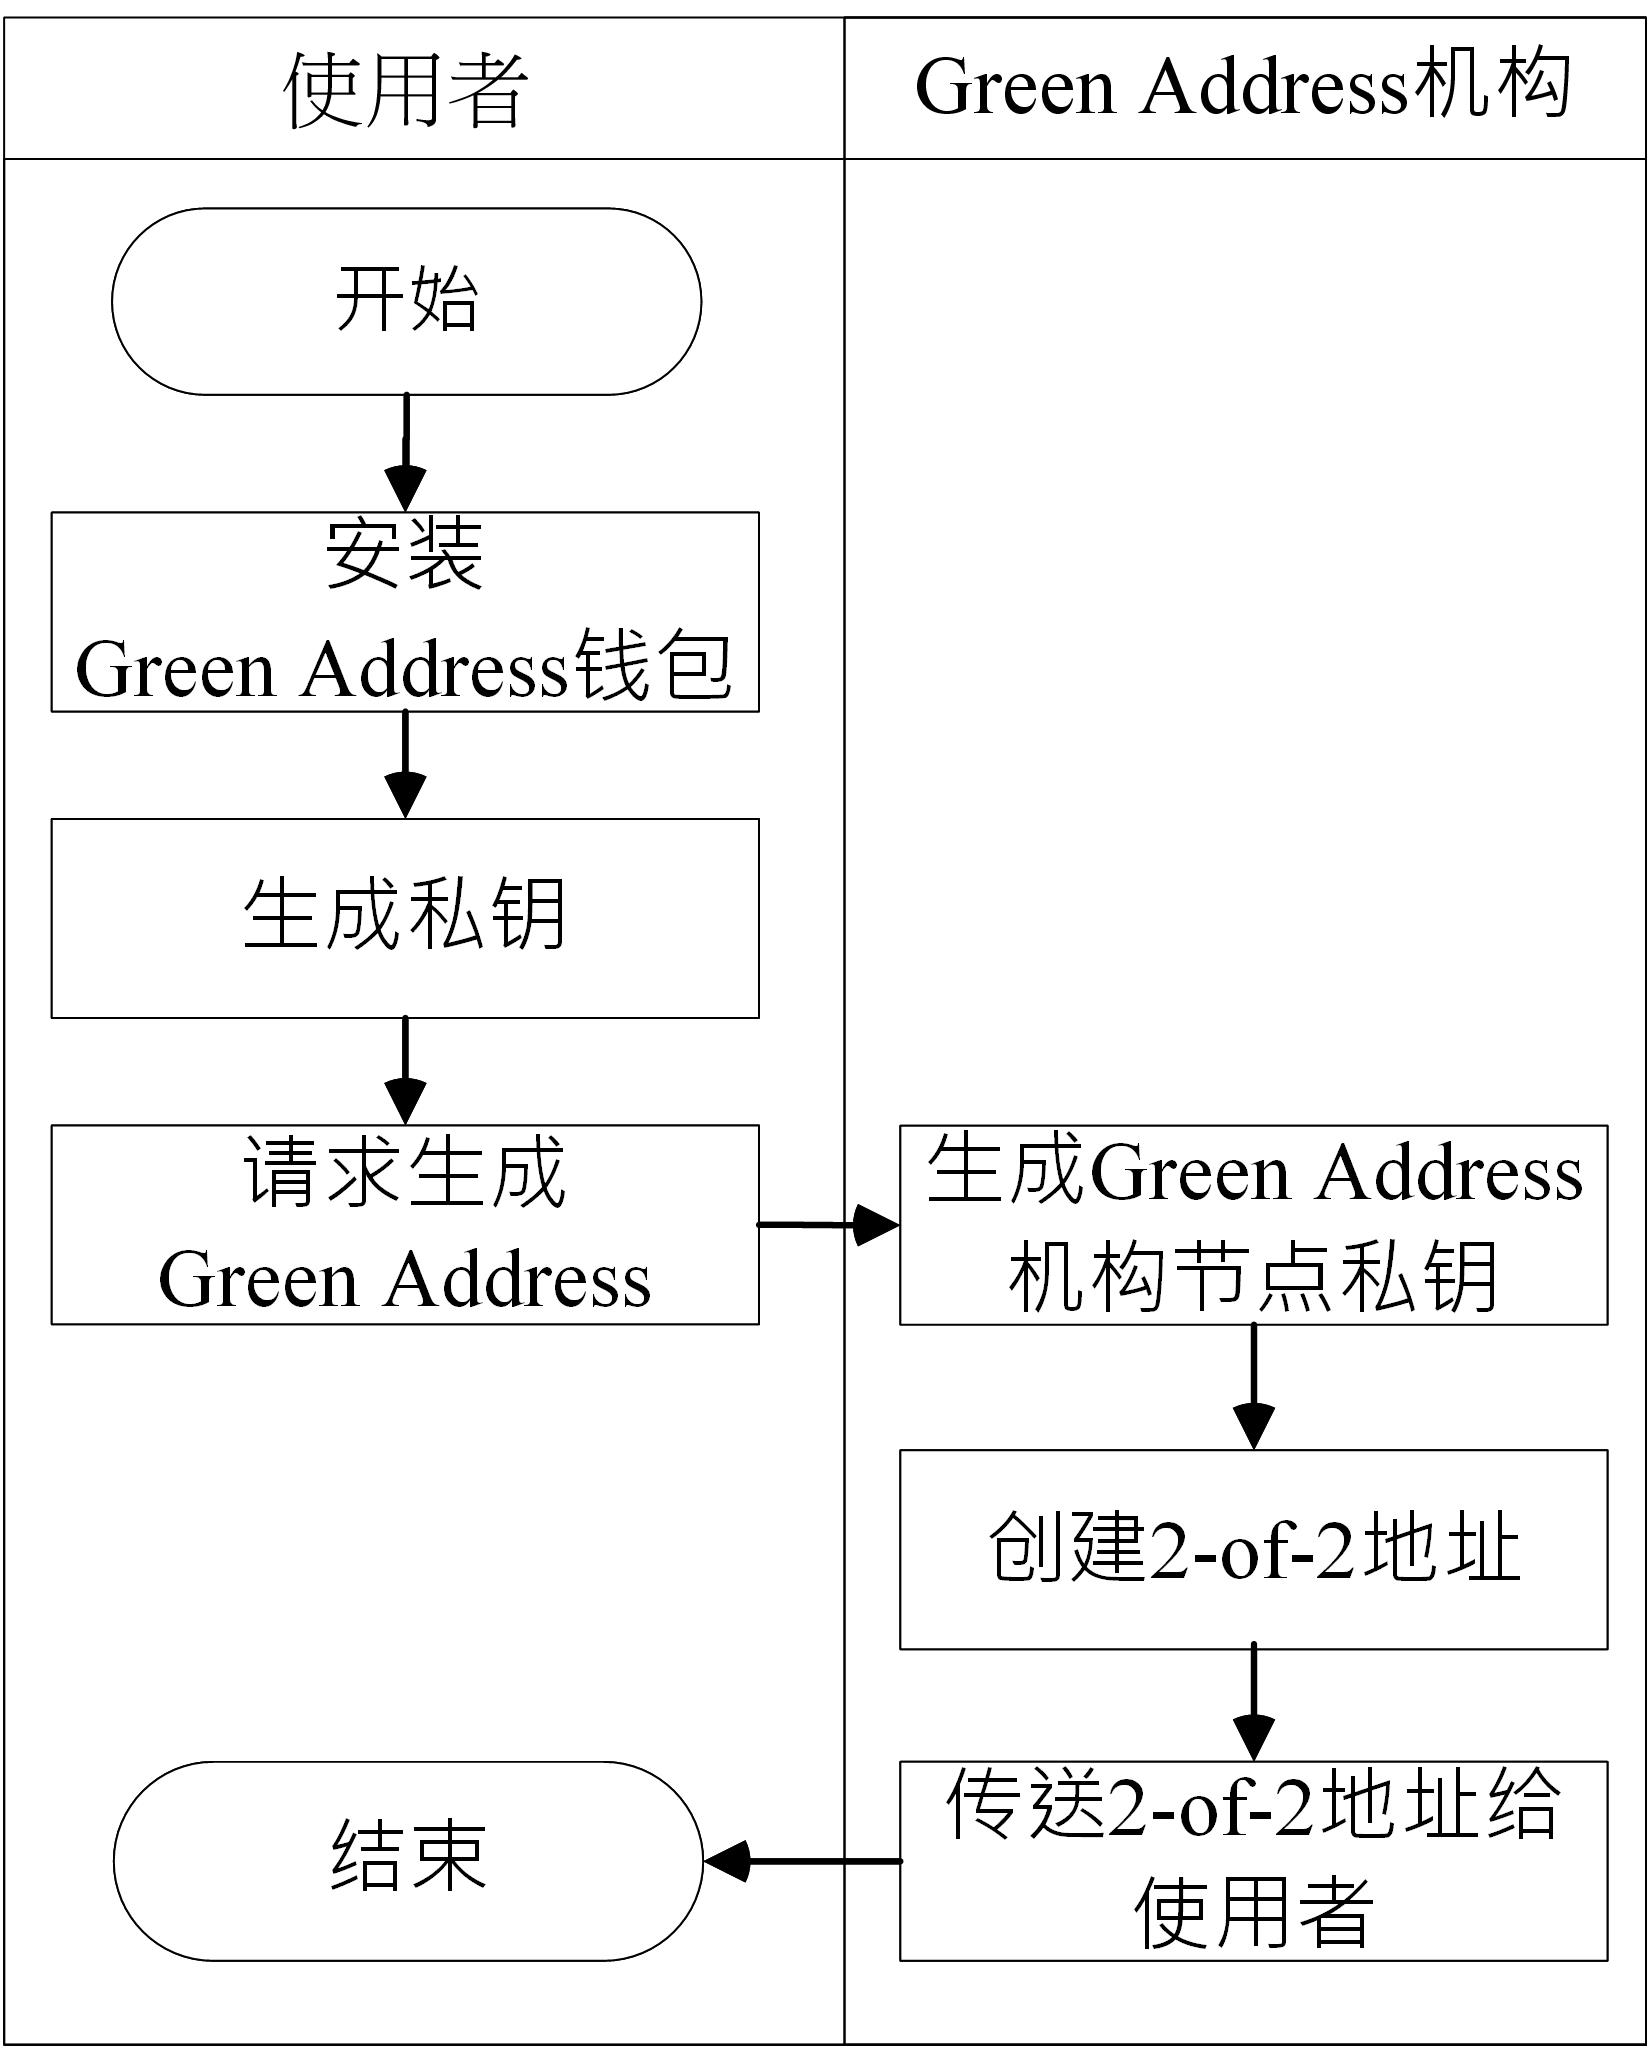
\includegraphics[width = .4\textwidth]{gabuild.jpg}
					\caption{Green Address钱包生成流程图}\label{gabuild}
				\end{figure}

			 	\begin{enumerate}
			 		\item 用户安装Green Address比特币钱包。
			 		\item 用户于本地端透过乱数产生器生成一个比特币私钥。
			 		\item 向Green Address机构节点请求创建2-of-2多重签章比特币地址。
			 		\item Green Address机构节点使用乱数产生器生成私钥。
					\item 创建2-of-2多重签章比特币地址如"2NGXNJrxq2qH6SuGEuJ57GjvMAmLUwPbZfQ",该地址的为多重签章地址,因此在地址的第一个字为"2",倘若为一般非多重签章地址,则地址的第一个字为"1"。
					\item 将生成的2-of-2多重签章比特币地址传回用户的Green Address比特币钱包。
			 	\end{enumerate}

			 	\subsubsection{(二)Green Address交易发起流程}
			 	说明完Green Address地址是如何创建之后,本节将详细说明如何运用多重签章地址发起交易至比特币网络中,如图\ref{gatx}所示。

			 	\begin{figure}[!htbp]
					\centering
					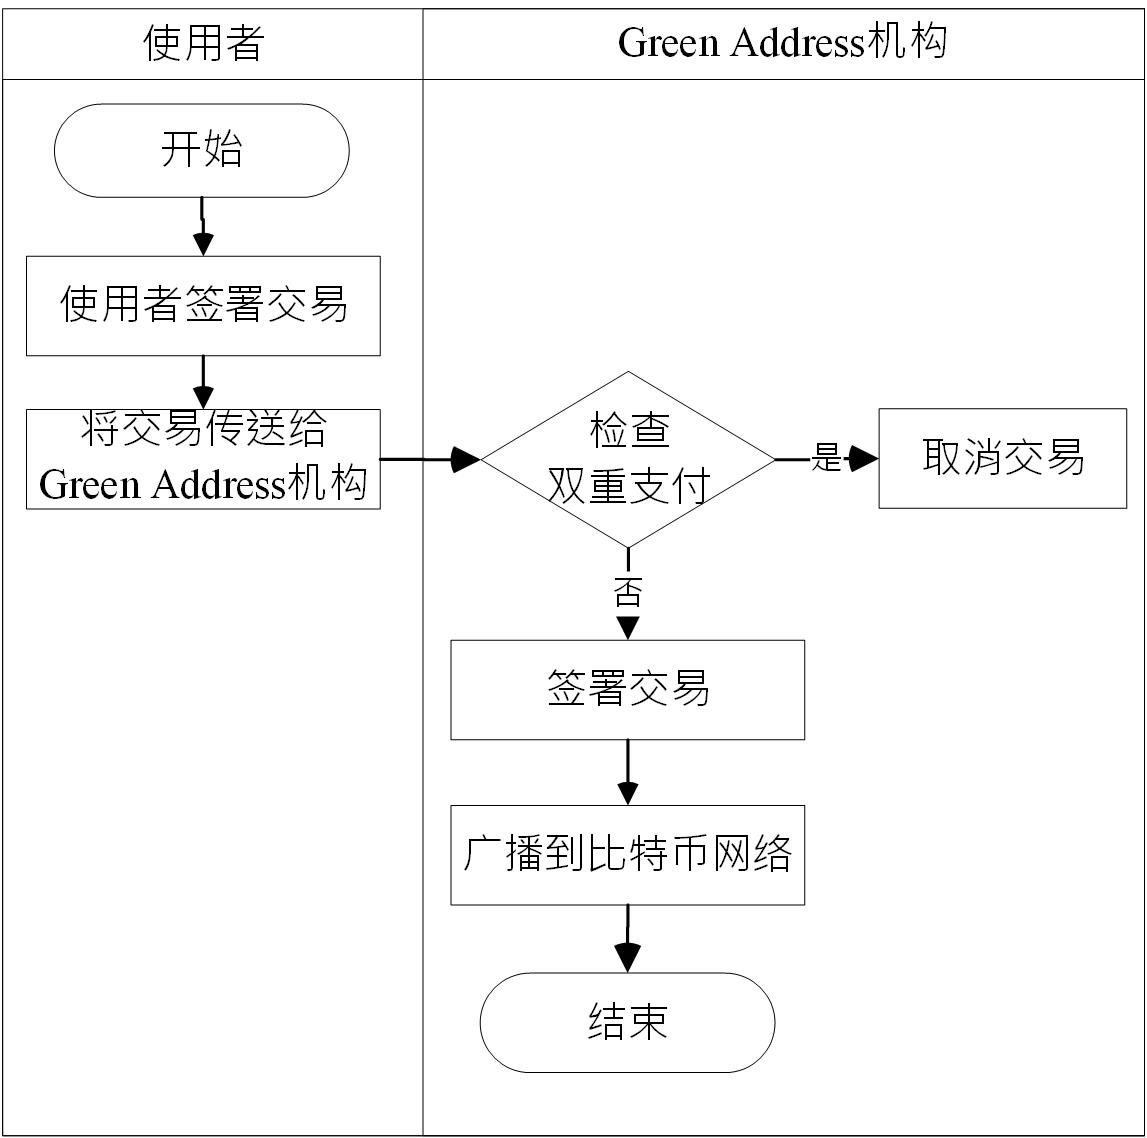
\includegraphics[width = .5\textwidth]{gatx.jpg}
					\caption{Green Address交易发起流程图}\label{gatx}
				\end{figure}

				\begin{enumerate}
					\item 用户使用原本创建Green Address的私钥,并完成签署交易。
					\item 因为是多重签章地址,所以该交易需发送至Green Address机构节点。
					\item Green Address机构节点收到交易信息后检查该交易的发起地址是否存在双重支付,倘若有双重支付则遗弃该笔交易;若无双重支付则往下一个步骤。
					\item Green Address机构以Green Address的私钥签署该笔交易。
					\item 将该笔交易封包广播至比特币网络。
				\end{enumerate}

		\section{区块链}
		%区块头所有的结构
		自2009年以来,加密货币比特币的诞生引发了新的货币革命浪潮,基于密码学,点对点网络,共识算法和区块链技术,它们被结合成比特币加密货币。到目前为止,它在九年内发生大量的袭击和欺诈事件后仍然在积极努力。 比特币一直是互联网上最具代表性的加密货币,同时是区块链技术极为重要的应用之一。
		比特币区块链可视为一种专门存储交易信息的数据库,该数据库的结构严谨。图\ref{blockchain} 為⽐特币区块链结构图,区块链之所以称为链是因为由许多区块构成,区块头存在于区块中记录区块中的重要信息共六项,分别为区块版本、前区块的哈希值、Merkle Root、难易度、时间戳以及Nonce,以下将逐一说明:

			\begin{figure}[!htbp]
				\centering
				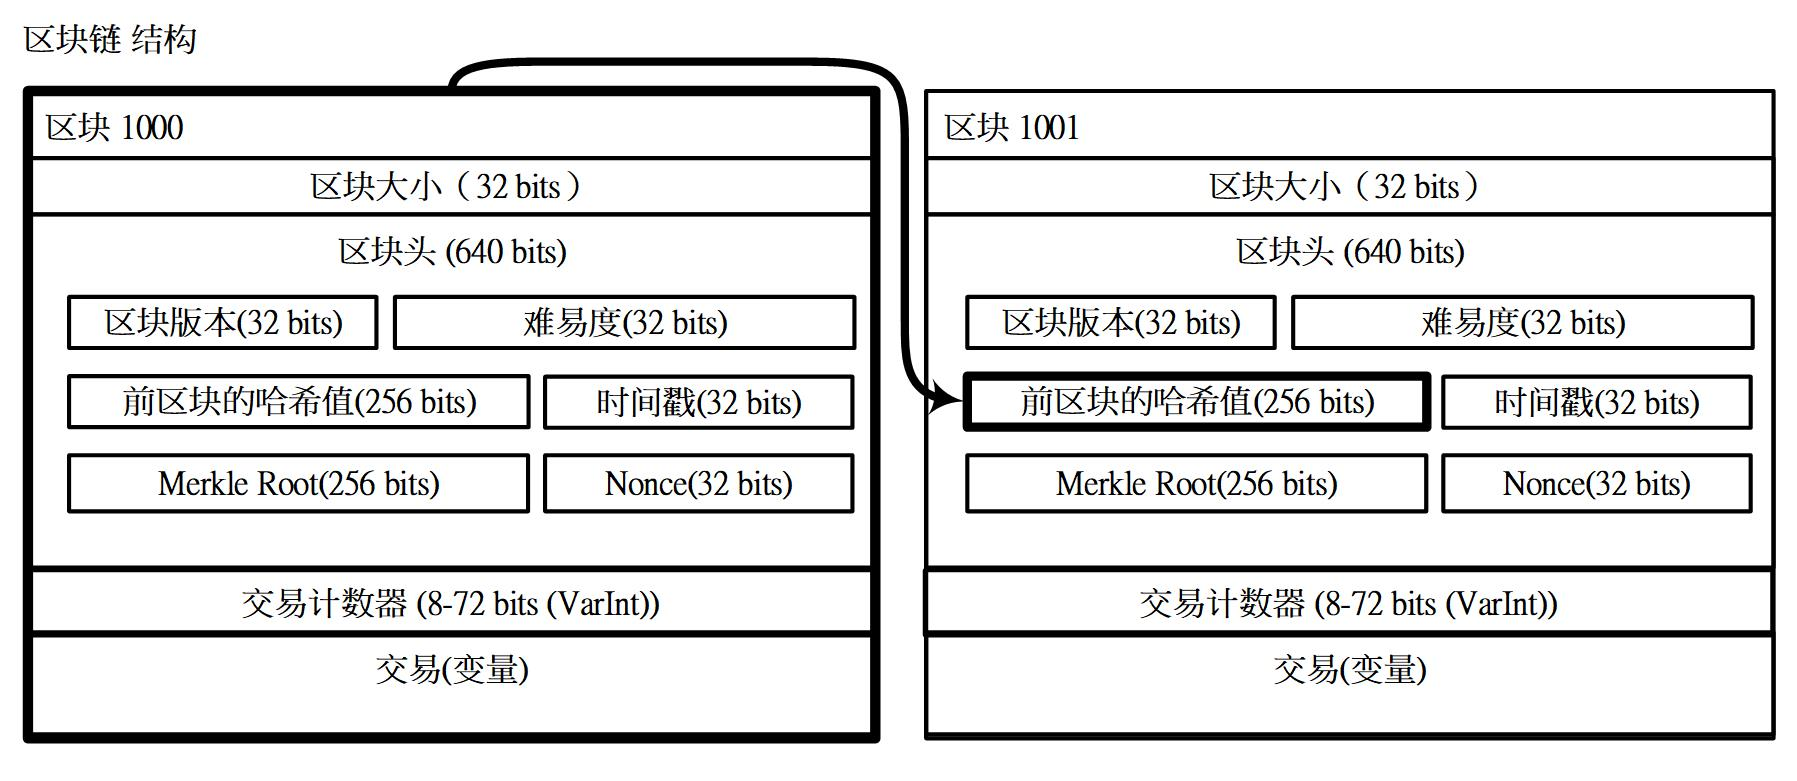
\includegraphics[width = 1\textwidth]{blockchain.jpg}
				\caption{比特币区块链结构图}\label{blockchain}
			\end{figure}

				\begin{enumerate}
				\item 区块版本(32 bits):该字段存储比特币区块链中的区块版本。
				\item 前区块的哈希值(256 bits):记录前一个区块的哈希值。 根据当前区块的前一个区块哈希值进而形成哈希指针,所有块可以因为哈希指针连接在一起形成比特币区块链,不仅可以在区块与区块间创建虚拟链结,还可以使得区块更难以被窜改。而通过新区块不断叠加在旧区块的过程,旧区块的哈希值将继续传递到最新的区块上。若区块上面堆叠更多的区块,促使哈希值的间接引⽤越多次,因此较早创建的区块更难以修改。

				\begin{figure}[!htbp]
					\centering
					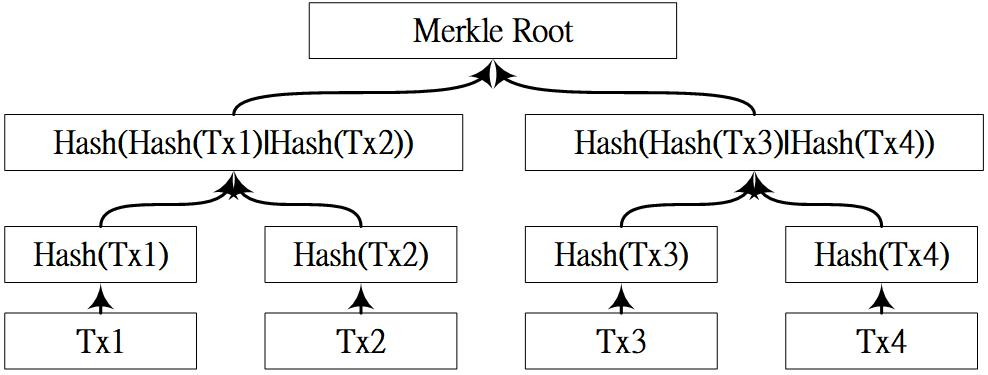
\includegraphics[width = 0.6\textwidth]{MerkleRoot.jpg}
					\caption{Merkle Tree示意图}\label{MerkleRoot}
				\end{figure}

				\item Merkle Root(256 bits):Merkle Root的生成方法是将当前区块的所有交易为$n$个进行排序后,Merkle Root为Merkle Tree的树根,交易为树叶$n$个,将每个树叶进行两次SHA-256 哈希算法取得哈希值得到$n$个哈希值,再将哈希值两两配对合并进行两次SHA-256 ,得到$n*2^{-1}$个哈希值后,在$k$轮后会使得$n*2^{-k}=1$时,合并到只剩下一个哈希值,最后一个哈希值则为Merkle Root,如图所示\ref{MerkleRoot},图中的Hash()函数为双重SHA-256 ,在区块链中的Merkle Root可用于快速检查当前区块中所有存储交易的正确性。

				

				\item 难易度(32 bits):难易度参数主要调控比特币挖矿过程中采用工作量证明算法的变量,值得一提的是比特币的难易度参数为动态调整。在过去加密货币的设计中,有着因为没有动态修改区块难度,而导致区块链生成速度太快,甚至导致区块链系统崩溃。
				\item 时间戳(32 bits):以年、月、日、小时、分钟和秒的格式记录区块生成时间。
				\item Nonce(32 bits):Nonce记录着矿工在进行挖矿时,必须要不断的尝试Nonce参数,直到符合难易度参数,才可以创建一个全新的比特币区块。该值为32 bits ,意为着矿工尝试的组态空间为$2^{32}$个可能性。
				\end{enumerate}
				
		%区块内容 交易手续费攻击
			%\subsection{Block Data}
			%	\subsubsection{交易计数器 (4-36 bits)}
			%	\subsubsection{交易信息}

		%\section{工作量证明(Proof of Work)}

		

		% \section{山寨币(Altcoin)简介}

		% 	\subsection{莱特币(Litecoin)}

		% 	\subsection{狗币(Dogecoin)}

		% 	\subsection{域名币(Namecoin)}

		% 	\subsection{以太坊(Etherum)}